\section{Skaitmeninės tapatybės valdymo apžvalga}

\subsection{Tapatybės patvirtinimo poreikis}

Šiais laikais naudotojo identifikavimas yra svarbi interneto taikomųjų
programų dalis. Paslaugų tiekėjai identifikuoja savo naudotojus norėdami \cite{RalucaBudiu2014}:

\begin{itemize}
    \item registruoti (angl. \textit{log}) naudotojų veiklą,
    \item užtikrinti, kad naudotojas iš tikrųjų yra asmuo, kuris sakosi esąs,
    \item suteikti dalį funkcionalumo tik autorizuotiems naudotojams,
    \item individualizuoti tinklalapio ar taikomosios programos turinį pagal naudotojo poreikius,
    \item sukurti paslaugos naudotojų bendruomenę,
    \item išvengti galimų anoniniminių naudotojų atakų.
\end{itemize}

Dėl išvardytų priežasčių naudotojų identifikavimas atlieka svarbią rolę įvairiose taikomųjų programų
srityse - elektroninėje valdžioje, elektroninėje komercijoje, verslo sumanume
(angl. \textit{business intelligence}), tyrimuose bei saugume
(angl. \textit{homeland security}) \cite{Glasser2009}. Kiekvienas paslaugų tiekėjas turi pasirinkti,
kaip autentifikuoti, ir, jei reikia, autorizuoti naudotojus. Programos kūrėjas taip pat turi saugoti
naudotojų suteiktus asmens duomenis ir užtikrinti jų saugumą, o naudotojui tenka rūpintis skirtingų turimų
paskyrų priežiūra ir savo duomenų sklaida tarp skirtingų sistemų. Minimus tapatybės atpažinimo
skaitmeninėje erdvėje aspektus nagrinėja skaitmeninės tapatybės valdymo disciplina.

\subsection{Skaitmeninės tapatybės valdymo samprata}

Dėl nuolat vykstančios interneto ir jame esančių paslaugų plėtros tapatybių
valdymo uždavinys pastaraisiais metais tapo itin svarbus \cite{Glasser2009}. Sprendžiant šį iššųkį,
sukurta skirtingų skaitmeninės tapatybės valdymo sistemų, siekiančių išspręsti naudotojų
tapatybės atpažinimo problemas. Šioms sistemoms įtaką daro
kiti tapatybę nagrinėjantys mokslai (pvz. sociologija), taip pat jos gali atlikti keletą skirtingų funkcijų, susijusių
su naudotojų tapatybe. Žemiau pateikiama diagrama,
kurioje pavaizduotas tapatybės valdymo sistemų kontekstas bei pagrindinės atliekamos užduotys:

\begin{figure}[H]
    \centering
    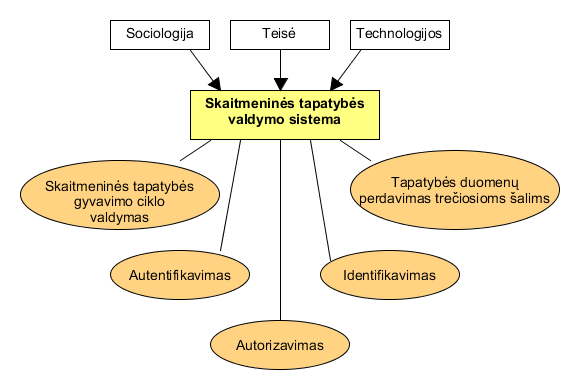
\includegraphics[scale=0.8]{img/IDMcontextAndUsecases}
    \caption{Skaitmeninių tapatybių valdymo sistemų kontekstas ir užduotys \cite{Glasser2009}}
    \label{img:mlp}
\end{figure}

Paveiksle matomos disciplinos turi skirtingą poveikį tapatybių valdymo sistemoms. 
Sociologija padeda apibrėžti tapatybę ir jos atitikmenį skaitmeninėje erdvėje, teisės mokslas nusako tapatybės duomenų naudojimo reikalavimus,
o esamos technologijos formuoja sistemos įgyvendinimo niuansus. Verta pastebėti, kad tapatybės valdymo sistema gali atlikti ne visas
diagramoje nurodomas funkcijas, o tik dalį iš jų. Taip pat, 1-ame paveiksle bei visame darbe naudojamos skaitmeninės tapatybės valdymo sąvokos,
tokios kaip \textit{identifikavimas}, \textit{autentifikavimas} ar \textit{autorizavimas} neretai suprantamos skirtingai, o tai sukelia
vieningos terminologijos trūkumą ir dėl jo kylančius neaiškumus \cite{Glasser2009}. Dėl to skyriuje
\enquote{Sąvokų apibrėžimai} pateikiami darbe dažniausiai naudojamų terminų aiškinimai.

Skirtingų tapatybių valdymo sistemo architektūros bei veikimo principai yra itin skirtingi - jie varijuoja nuo
lokalaus autentifikavimo kiekvienai programai iki centralizuotos platformos, dedikuotos tik konkrečiai
tapatybės atpažinimo funkcijai. S. Clauß ir M.Köhntopp savo tyrime pastebi, kad nėra vieningo standarto identiteto
valdymo sistemoms \cite{Claus2001}. Tolesniuose skyriuose pateikiamos skirtingos technologijos
bei sprendimai, naudojami skaiteminių tapatybių valdyme, jų privalumai bei trūkumai.